\chapter{Statistical Inference}
\label{chp:statisticalinference}

\begin{multicols}{2}[\subsubsection*{Contents of this chapter}]
   \printcontents{}{1}{\setcounter{tocdepth}{2}}
\end{multicols}

\section{Parametric and Nonparametric Models}

A statistical model $\mathfrak{F}$ is a family of functions. \textit{Parametric models} can be parametrized by a finite number of parameters. For example, the Gaussian Normal distribution $\mathscr{\mu,\sigma^2}$ has the two parameters $\mu$ and $\sigma^2$. The general form is:

\begin{equation}
\mathfrak{F} = \{f(x;\theta): \theta \in \Theta \}
\end{equation}

Where $\theta$ is a vector of parameters and $\Theta$ is the parameter space. Elements of $\theta$ that are not of interest are called \textit{nuisance parameters}. \textit{Nonparametric models} cannot be described by a finite number of parameters. An example is an interpolating spline.


% fundamental concepts
\section{Fundamental Concepts in Inference}


% point estimations
\subsection{Point Estimation}
Point estimation refers to providing a single best guess of some quantity of interest. The point estimator is denoted with a had, i.e. $\hat{\theta}$. The point estimator for some quantity based on $n$ datapoints:

\begin{equation}
\hat{\theta}_n = g(X_1,X_2,...,X_n)
\end{equation}


% bias
\subsection{Bias}
A point estimator $\hat{\theta}$ has bias:

\begin{equation}
\mathrm{bias}(\hat{\theta}_n) = \mathbb{E}_\theta (\hat{\theta}) - \theta
\end{equation}

Where $\theta$ is the "true" value $\theta_n \rightarrow \theta$ as $n \rightarrow \infty$. $\mathbb{E}_{\theta}(r(X)) = \int r(x) f(x;\theta) \mathrm{d}x$. 

% consistency
\subsection{Consistency}

A point estimator $\hat{\theta}_n$ is consistent if $\hat{\theta}_n \xrightarrow{P}\theta$. That is, it converges in probability to $\theta$. $\hat{\theta}_n$ is consistent with both bias and standard error approach $0$ as $n\rightarrow \infty$.


\subsection{Sampling Distribution, Standard Error}

The distribution of $\hat{\theta}_n$ is the \textit{sampling distribution}. The standard deviation of the distribution of $\hat{\theta}_n$ is the \textit{standard error}, denoted $\mathrm{se}$. 

\begin{equation}
\mathrm{se}(\hat{\theta}_n) = \sqrt{\mathbb{V}(\hat{\theta}_n)}
\end{equation} 

The standard error might depend on the unknown population CDF, in which case it is estimated. The point estimator for the standard error is then $\hat{\mathrm{se}}$. 



\subsubsection{Example: Bernoulli Distribution}

Let $X_1,X_2,X_3 \sim \mathrm{Bernoulli}(p)$. The point estimator for $p$ based on $n$ datapoints is $\hat{p}_n = \frac{1}{n}\sum_{i=1}^n X_i$. Then the expected value of the point estimator $\mathbb{E}(\hat{p}_n) = \frac{1}{n}\sum_{i=1}^n \mathbb{E}(X_i) = p$, so that $\hat{p}_n$ is unbiased. The standard error is $\mathrm{se} = \sqrt{\mathbb{V}(\hat{p}_n)} = \sqrt{\frac{p(1-p)}{n}}$. The estimated standard error is $\hat{\mathrm{se}} = \sqrt{\frac{\hat{p}(1-\hat{p})}{n}}$.


% MSE
\subsection{Mean Squared Error}
The quality of a point estimator is often measured using the \textit{mean squared error}:

\begin{equation}
\mathrm{MSE} = \mathbb{E}_{\theta}(\hat{\theta}_n - \theta)^2 = \mathrm{bias}^2(\hat{\theta}_n) + \mathbb{V}_{\theta}(\hat{\theta}_n)
\end{equation}


% Asymptotically Normal
\subsection{Asymptotically Normal Estimators}
An asymptotically normal estimator satisfies:

\begin{equation}
\frac{\hat{\theta}_n - \theta}{\mathrm{se}} \xrightarrow{dist} \mathscr{N}(0,1)
\end{equation}


% confidence sets
\subsection{Confidence Sets}

A confidence set $C_n$ is the subset of parameters $\theta$ that has a greater than $1-\alpha$ probability of containing the true value of $\theta$.

\begin{equation}
\mathbb{P}_{\theta}(\theta \in C_n)\geq 1-\alpha\ \mathrm{\ for\ all\ }\theta\in\Theta
\end{equation}

\subsubsection{Normal-Based Confidence Intervals}

If $\hat{\theta}_n \approx \mathscr{N}(\theta,\hat{\mathrm{se}}^2)$ and $z_{\frac{\alpha}{2}} = \Phi^{-1}(1-\frac{\alpha}{2})$ the value of the standard normally distributed random variable $Z$ at which $\mathbb{P}(-\frac{\alpha}{2} < Z < \frac{\alpha}{2}) = 1-\alpha$, then, transforming backwards, $\mathbb{P}(\hat{\theta}_n - z_{\frac{\alpha}{2}}\hat{\mathrm{se}} < \theta < \hat{\theta}_n + z_{\frac{\alpha}{2}}\hat{\mathrm{se}} ) = 1-\alpha$. Hence, the confidence interval for a normally distributed point estimator $\hat{\theta}_n$ is: 

\begin{equation}
C_n = (\hat{\theta}_n - z_{\frac{\alpha}{2}}\hat{\mathrm{se}},\hat{\theta}_n + z_{\frac{\alpha}{2}}\hat{\mathrm{se}})
\end{equation}

For a 95\% confidence interval $\alpha=0.05$ and $z_{\frac{\alpha}{2}} = 1.96 \approx 2$, so that the confidence interval is approximately $\hat{\theta}_n \pm 2 \hat{\mathrm{se}}$. 


\subsubsection{Pointwise and Uniform Asymptotic Confidence Intervals}

A \textit{pointwise asymptotic} confidence interval requires:

\begin{equation}
\liminf_{n\rightarrow \infty} \mathbb{P}_{\theta}(\theta \in C_n) \geq 1-\alpha,	\ \ \forall \theta \in \Theta
\end{equation}   

A \textit{uniform asymptotic} confidence interval requires:

\begin{equation}
\lim_{n\rightarrow \infty}\inf_{\theta \in \Theta} \mathbb{P}_{\theta}(\theta \in C_n) \geq 1-\alpha
\end{equation}



\section{Non-Parametric Estimation of the CDF and Statistical Functionals}

\subsection{Empirical Distribution Function}
It may be necessary to perform non-parametric estimation of the CDF $F$ of a set of random variables $X_1, X_2, ... , X_n \sim F$. 

The empirical distribution function $\hat{F}_n$ is the CDF that puts mass $1/n$ at each point $X_i$.

\begin{equation}
\hat{F}_n(x) = \frac{\sum_{i=1}^n I(X_i \leq x)}{n}
\end{equation}

Where $I(X_i \leq x) = \left\{\begin{array}{c} 1\ \mathrm{if\ } X_i \leq x\\ 0\ \mathrm{if\ } X_i > x \end{array} \right.$. 

The empirical CDF is discrete, even when the random variable it is based on may be continuous. 

At a given point $x$, $\hat{F}_n(x)$ is an unbiased estimator of $F(x)$. 

\begin{itemize}
\item $\mathbb{E}\hat{F}_n(x) = F(x)$
\item $\mathbb{V}\hat{F}_n(x) = 0+\mathrm{MSE} = \frac{F(x)(1-F(x))}{n}$
\item $\hat{F}_n(x) \xrightarrow{P} F(x)$
\end{itemize}

The Glivenko-Cantelli Theorem guarantees that, if $X_1,X_2,...,X_n \sim F$, then:

\begin{equation}
\sup_x |\hat{F}_n(x) - F(x)|\xrightarrow{P} 0
\end{equation}

\subsection{Confidence Measures for the Empirical CDF}
A confidence interval for the empirical CDF is given through the Dvoretzky-Kiefer-Wolfowitz (DKW) Inequality:

\begin{equation}
\mathbb{P}\left(\sup_x|F(x) - \hat{F}_n(x)|>\epsilon \right)\leq 2 e^{-2n\epsilon^2}
\end{equation}

A nonparametric $1-\alpha$ confidence band is then:

\begin{equation}
\begin{array}{c}
L(x) = \max\{\hat{F}_n -\epsilon_n, 0 \}\\
\\
U(x) = \min\{\hat{F}_n + \epsilon_n, 1\}
\end{array}
\end{equation}

with $\epsilon_n = \sqrt{\frac{1}{2n}\log\left(\frac{2}{\alpha}\right)}$.

\begin{equation}
\mathbb{P}\left(L(x) \leq F(x) \leq U(x) \right) \geq 1-\alpha
\end{equation}
	


\subsection{Statistical Functionals}
A functional is, roughly speaking, a function of a function. The fourier transform of a function is a functional. A \textit{statistical functional} is any function of the CDF, $F$. Examples are the mean, the variance, or the median. 

\subsection{Plug-in Estimator}
The plug-in estimator of $\theta = T(F)$ is given by $\hat{\theta} = T(\hat{F}_n)$. In other words, the estimate of the CDF is used instead of the true $F$, resulting in an estimator.

\subsection{Linear Functionals}
Functionals of the form $T(F) = \int r(x) dF(x)$ are linear functionals.  

\subsection{Plug-in Estimator for Linear Functionals}
\begin{equation}
T(\hat{F}_n) = \int r(x) d\hat{F}_n(x) = \frac{1}{n}\sum^{n}_{i=1}r(X_i)
\end{equation}

\subsection{Examples: Mean, Variance, Sample Variance, Sample Correlation}
\citeasnoun{wasserman2013all} pp. 100


\section{The Bootstrap}

Bootstrap allows for investigating the variance of a statistic by calculating the statistic many times on samples drawn from the empirical CDF. This amounts to sampling from the dataset with replacement (i.e. datapoints may be included in a sample several times).

There are two approximations in play: first, the true CDF is approximated using the empirical CDF. Second, the variance of the statistic is estimated based on a sample.

Uncertainty in terms of bootstrap estimates may be calculated in terms of normal, pivotal or percentile intervals. The normal interval is valid when the statistic is approximately normally distributed.

\section{Jackknife}
The Jackknife method is less computationally expensive, but less general than the bootstrap. For a dataset of $n$ elements, the Jackknife method calculates the statistic $n$ times, each time removing one of the estimates from the calculation. The jackknife does not produce consistent estimators of the standard error of sample quantiles. 


\section{Parametric Inference}

In parametric inference, the quantity of interest might be some function $T(\theta)$. The sought-after parameters are \textit{parameters of interest} and additional parameters that emerge as part of the model are \textit{nuisance parameters}. Parametric inference deals with creating parametric estimators.

\subsection{Method of Moments}
The method of moments relies on a system of linear equations to link estimators of moment to sample moments. The $j$th moment is given by:

\begin{equation}
\alpha_j = \int x^j dF_{\theta}(x)
\end{equation}

The $j$th sample moment is given by:

\begin{equation}
\hat{\alpha}_j = \frac{1}{n} \sum_{i=1}^ n X_i^j
\end{equation}


The method of moments estimator $\hat{\theta}_n$ is defined to be the value of $\theta$ so that:

\begin{equation}
\begin{array}{l}
\alpha_1(\hat{\theta}_n) = \hat{\alpha}_1\\
\alpha_2(\hat{\theta}_n) = \hat{\alpha}_2\\
\alpha_3(\hat{\theta}_n) = \hat{\alpha}_3\\
\alpha_4(\hat{\theta}_n) = \hat{\alpha}_4\\
\vdots
\end{array}
\end{equation}

The method of moments estimator satisfies:

\begin{enumerate}
\item The estimate $\hat{\theta}_n$ exists with probability tending to 1.
\item The estimate is consistent: $\hat{\theta}_n \xrightarrow{P}\theta$ (it converges in probability)
\item The estimate is asymptotically normal (cf. \cite{wasserman2003all}, pp.122)
\end{enumerate}


\subsection{Maximum Likelihood Estimation}

The maximum likelihood estimator is the value $\hat{\theta}$ that maximizes the joint probability density of the data, called the likelihood function. 

For i.i.d. random variables with pdf $f(x;\theta)$, the likelihood function is:

\begin{equation}
\mathscr{L}_n(\theta) = \prod_{i=1}^n f(X_i;\theta)
\end{equation}

And the log likelihood functin is $l_n(\theta) = \log \mathscr{L}_n(\theta)$. Since $\log$ is a monotonic function, maximizing the log-likelihood yields the same estimator as maximizing the likelihood directly. Log-likelihood is often easier to deal with, and alleviates numerical issues associated with the often sharply spiked likelihood function. 

MLE estimators have a flurry of desirable properties under certain smoothness conditions on the density function. 

\begin{itemize}
\item Consistency: convergence in probability upon the true value
\item Equivariance: if $\hat{\theta}_n$ is the MLE of $\theta$ then $g(\hat{theta}_n)$ is the MLE of $g(\theta)$
\item Asymptotically Normal
\item Asymptotically Optimal / Efficient: smallest variance, at least for large samples.
\item Approximately the Bayes estimator.
\end{itemize}


\subsection{Parametric Confidence Intervals}

Confidence intervals for infered parameters in the parametric setting can be derived, for example, using the delta method (assuming that the estimators are asymptotically normal) or using parametric bootstrap. In the nonparametric case, bootstrap sampled from the empirical CDF. In the parametric case, bootstrap sample from the density $f(X;\hat{\theta})$ where $\hat{\theta}$ is the estimator.


\section{Score Function, Fisher Information}
Given some pdf $f(X;\theta)$, the score function is given by: 

\begin{equation}
s(X;\theta) \frac{\partial \log f(X;\theta)}{\partial \theta}
\end{equation}

The Fisher information is the variance of the score function at each datapoint:

\begin{equation}
I_n(\theta) = \mathbb{V}_{\theta} \left(\sum_{i=1}^n s(X_i ; \theta) \right)
\end{equation}





\section{Directional Statistics}

\subsection{Mean Direction}
The mean direction of a collection of $i$ vectors $\{\mathbf{x}\}_i$ is \cite{damask2019consistent}:

\begin{equation}
\left<\mathbf{x}\right> = \frac{\mathbf{x_s}}{||\mathbf{x_s}||_2}
\end{equation}

Where

\begin{equation}
\mathbf{x_s} = \sum_i \mathbf{x_i}
\end{equation}

The mean vector is not defined in case $||\mathbf{x_s}||_2 = 0$. The alternative way to calculate the mean direction might make use of angles but apparently that creates ambiguity with respect to the choice of a "zero" angle (cf. footnote in \citeasnoun{damask2019consistently}).



\subsection{Dispersion}

Dispersion is a measure of the variance on the direction of a set of vectors $\{\mathbf{x}\}_i$. For a system of vectors, for example an eigenbasis, both common and differential modes of estimation exist. One way of meausuring directional dispersion is to look at the \textit{mean resultant length}:

\begin{equation}
\mu_r = \frac{||\mathbf{x_s}||}{N}\ \ \ 0\leq \mu_r \leq 1
\end{equation}

\textit{Circular variance} may be defined as $\sigma_c = 1-\mu_r$, but apparently there is an issue with generalization to higher dimensions. (TO DO)

An alternative is a model based approach, for example based on the von Mises - Fisher Distribution.

In the case of a basis, \citeasnoun{damask2019consistently} states that, in order to understand the drivers for variation, dispersion parameters should be calculated for each descending subspace of the basis, first including all of the eigenvectors, then excluding the first eigenvector, etc.





\section{Features}

Features are sources of information that hopefully allow conclusions towards some kind of quantity of interest. Some people like to call them independent variables.

\subsection{Dense Features, Sparse Features}
Sparsity and density refer to the fraction of a matrix that is zeros. In the context of features, sparse features typically refer to feature vectors that have many zeros in them. I.e., $[1,2,5,2,6,3,0]$ would be a dense feature vector and $[2,0,0,0,0,3,0,0,1]$ would be a sparse feature vector. Typically, sparsity is touted as an advantage because it allows for lossless compressed representations of high-dimensional data, which has computational advantages. Another advantage, though, is that sparse representations can be more interpretable by containing information in an inherently more condensed fashion. They are also thought to prevent overfitting: many regularization techniques aim to minimize the number of parameters or features used in a predictive model, which amounts to biasing an algorithm towards learning sparse coefficients. An example is ridge regression. 

\section{Multicollinearity}
So far this section is based on \citeasnoun{ncssridgeregression}.

Multicollinearity, or collinearity, occurs when features are linearly correlated with each other. The effects are horrible. They include inaccurate estimates of the regression coefficients, higher standard errors of the regression coefficients, lower partial t-tests for the regression coefficients, falsely insignificant p-values and decreased predictive power of the model. And other things.

\subsubsection{Detection}

\subparagraph{Scatter Plots}
Scatterplots provide a visual test for collinearity by hopefully exposing relationships between independent variables. This is subjective and unreliable, but people love plots.

\subparagraph{Variance Inflation Factors (VIF)}
A VIF over 10 it said to indicate collinear variables.

\subparagraph{Eigenvalues of the Correlation Matrix}
Linear relationships between two or more variables cause the corresponding rows of the correlation matrix to be identical or very similar. Correspondingly, the matrix will be singular or near-singular, which will manifest itself through zero or near-zero eigenvalues. The conditioning number, given by the largest eigenvalue divided by the smallest eigenvalue, are a quick way to test for this. A large conditioning number indicates collinearity.

\subparagraph{Regression Coefficients}
Collinearity increases the standard error of the regression coefficients because it allows for the variation of the dependent variable to be explained in terms of a greater variety of different weights assigned to the collinear variables. Counterintuitive results for the regression coefficients may be the result of collinearity. 

\subsection{Sources}

\subparagraph{Data Collection}
\subparagraph{Physical Constraints}
\subparagraph{Over-defined Model}
\subparagraph{Model Choice or Specification}
\subparagraph{Outliers}

\subsubsection{Remedies}

\subparagraph{Dimensionality Reduction}
SVD, PCA, NNMF and other dimensionality reduction techniques allow for the feature space to be shrunk in a way that aims to optimally preserve information. Any technique worth its salt will either collapse or filter collinear variables into a reduced-rank representation of the information in the dataset.

\subparagraph{Regularization}
Certain forms of regularization are similar in spirit to dimensionality reduction, except that, rather than addressing the dataset, they reduce the parameters used by a model to fit to the data. The canonical example is ridge regression. Ridge regression penalizes the use of a larger number of parameters and, if two variables are collinear, will tend to push the weight of one of them towards zero. It is important to standardize the variables before fitting the model, so that the regression weights for different variables are on the same scale. Ridge regression remains controversial \cite{ncssridgeregression}. 


\section{Fat Tails}
Roughly speaking, the consequences of ``fat tails" is that rare events tend to play a disproportionally large role in determining the statistical properties of a sample. This is in contrast to ``thin tails", where, as the sample size increases, pretty quickly no single observation modifies the statistical properties of the sample.

For ``thin tails", extreme observations tend to result from the combination of several very unlikely events. For ``fat tails", an extreme observation tend result from a single very unlikely event. 

\subparagraph{Thin Tails}
Two people are randomly selected, and their combined height is 4 meters. Most likely this resulted from the selection of two people who are two meters tall, rather than one person that is 10 cm and another that is 3,90 m tall. 

\subparagraph{Fat Tails}
Two people are randomly selected, and their combined net worth is \$ 40M. The probability of having selected two people with a net work of \$ 20M is less likely than having selected one person with a net worth of \$ 200k and another person with a net worth of \$ 39,8 M. 

Fat tails do not imply that rare events are more frequent, but that they have greater impact when they do happen. In fact, ``fattening" the tails of a Gaussian distribution results in a larger number of observations within one standard deviation. 

\begin{figure}
\centering
    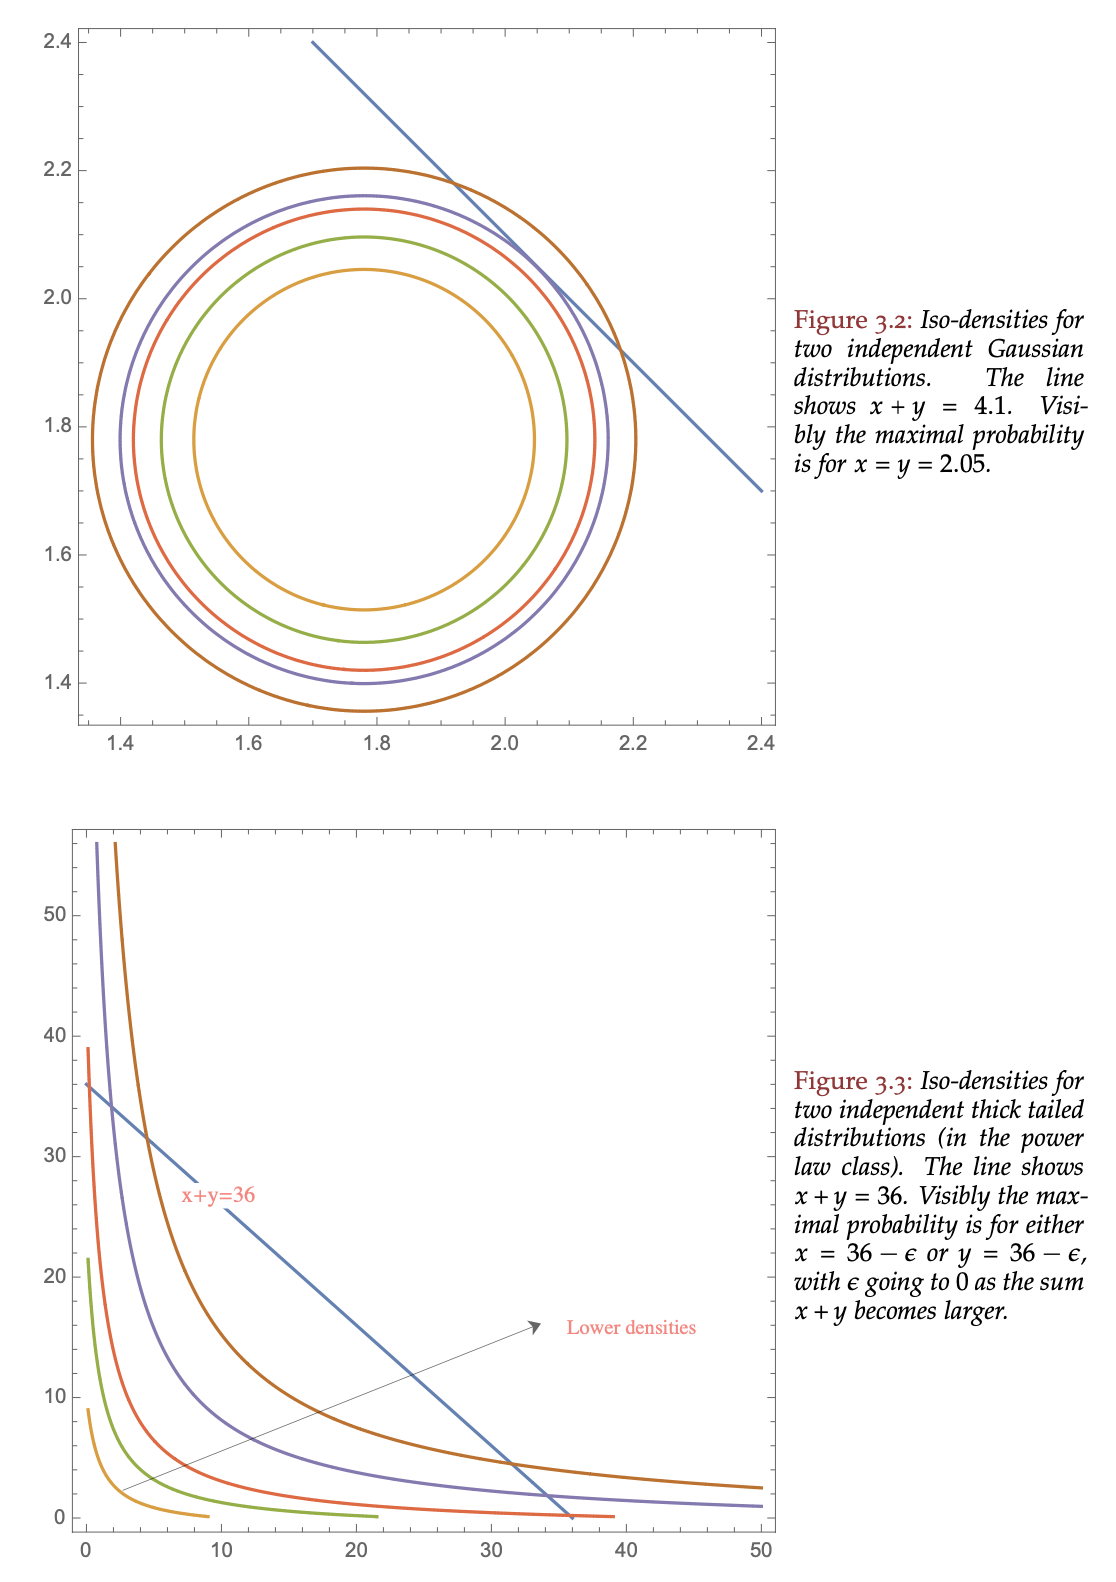
\includegraphics[width=\textwidth]{fattails01.png}
    \caption{Probability densities of two independent thin tailed and thick tailed random variables (brazenly copied from Taleb, 2020). Compare to plot of Lp norms. For the thin tailed random variables, the observa- tion of a particular sum is most likely to result from a balanced contribution from both random variables. For the fat tailed random variables, the observation of a particular sum is most likely to result from the contribution of one of the variables.}
    \label{fig:fattails01}
\end{figure}

\subsection{Consequences of Fat Tails}

\subparagraph{The Law of Large Numbers works too Slowly}

\subparagraph{The Sample Mean will rarely correspond to the Distribution Mean}
For example, for an 80/20 power law, 92\% of the observations will fall below the distribution mean. The sample mean will tend to underestimate the distribution mean because the distribution mean is heavily biased by rare observations that will tend to be underrepresented in the sample.

\subparagraph{Metrics such as Sample Mean and Sample Variance will be Unusable}

\subparagraph{In finance, metrics like Sharp etc. are unusable}

\subparagraph{Gauss-Markov Theorem fails}
Therefore, linear least squares regressions do not work. 

\subparagraph{Maximum Likelihood Methods can still work}
For example in case of a Pareto distribution, it is possible to fit the tail exponent using maximum likelihood methods, and estimating the mean from there. Direct observation of the mean would be misleading. The tail exponent intelligently extrapolates the fat tails of the distribution.

\subparagraph{Absence of Evidence $\neq$ Evidence of Absence}

\subparagraph{PCA is going to cause spurious factors and loads}

\subparagraph{Method of Moments does not work}
Approximating a distribution by matching its moments does not work when higher moments are undefined or cannot be reliably estimated.

\subparagraph{There is no ``typical" large deviation}


\subsection{Maximum to Sum}
The "maximum to sum" or MS plot allows to see the behavior of the relationship between the observed maximum to the sum for a particular moment as the number of observations increases. 

\subsection{Maximum Domain of Attraction}

The ``maximum domain of attraciton" is, so to speak, the ``right endpoint of the distribution":

\begin{equation}
x^* = \sup\{x: F(x) < 1 \}
\end{equation}

\subsection{Hidden Tail, Problems in Estimating Moments}
The Glivenko-Cantelli theorem guarantees uniform convergence of the empiral cdf to the true CDF, however, the empirical distribution is necessarily bounded by the values of the minimum and maximum observations. This results in an unobserved contribution to moments $p>0$ that does not necessarily have to be negligible. To illustrate, take $K_n$ to be the maximum observed value. 
\begin{equation}
\mathbb{E}(X^p) = \underbrace{\int_{L}^{K_n} x^p \phi(x)\mathrm{d}x}_{observed} + \underbrace{\int_{K_n}^{\infty} x^p \phi(x)\mathrm{d}x}_{unobserved}
\end{equation}






\section{$R^2$ Value}

\section{Regression Diagnostics}

\section{t-Statistics}

\section{AIC and BIC}

\section{Factor Regression}

\section{Factor Models}


\section{How to Combine Estimates with Different Uncertainties}
A series of classic papers exist on this subject.  


\section{How to Tackle Very High Dimensional Feature Spaces}
In practice, high-dimensional feature spaces amplify the risk of overfitting. The answer, framed in the most general way, is to introduce limitations on the family of functions that are fit by the estimator of choice. The generic methods are regularization (i.e. penalizing variance), variable selection (i.e. filtering out irrelevant features) and dimensionality reduction through feature transformation (i.e. finding a lower-rank representation of the data). It's not possible to draw neat distinctions between this methods in terms of their effects. For example, regularization often amounts to variable selection through soft (or hard) thresholding. Drop out regularization in neural networks biases the model towards particular types of feature transformations.



